% -- Slide ---------------------------------------------------------------------
\begin{frame}
\frametitle{\bf Backend Overview}

% \begin{itemize}
%     \item Basic block ordering
%     \item Register allocation (linear scan)
%     \begin{itemize}
%         \item Instruction numbering and intervals
%         \item Hints
%     \end{itemize}
%     \item Operand assignment
%     \item SSA deconstruction
%     \item Translation
%     \item Linking and assembly
% \end{itemize}
\begin{center}
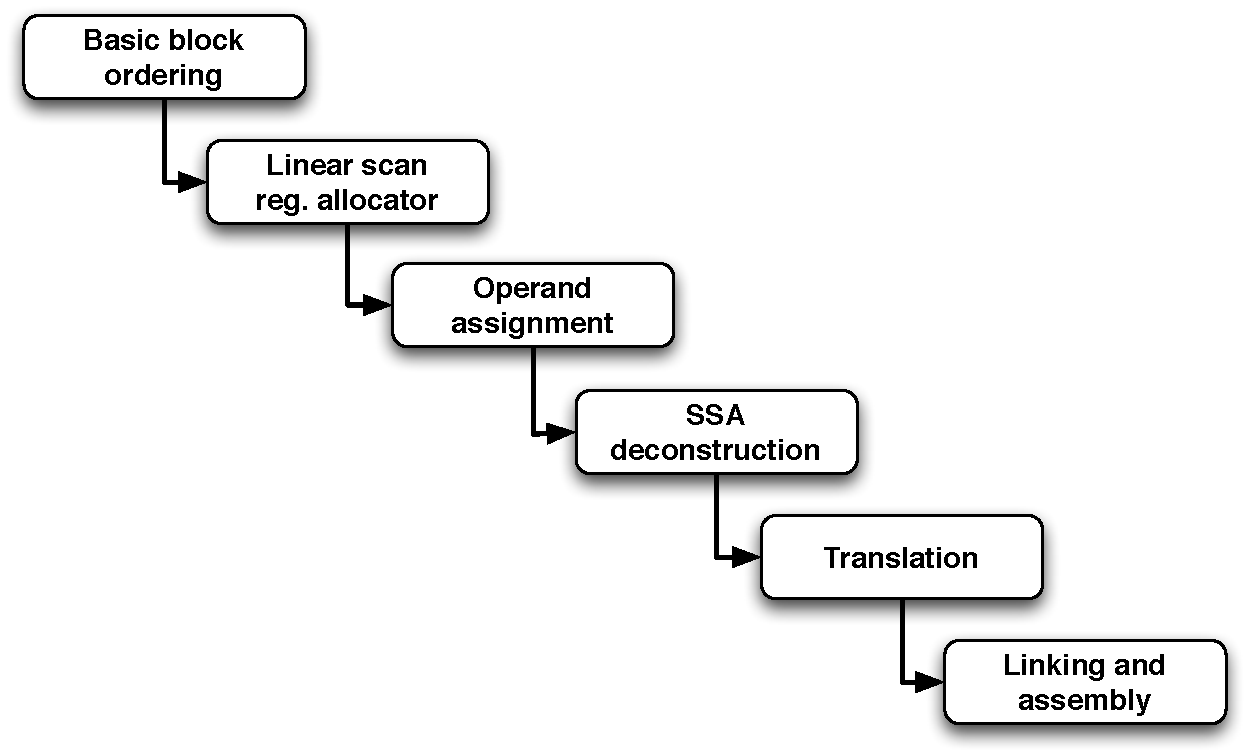
\includegraphics[width=4in]{images/backend}
\end{center}
\end{frame}
% ------------------------------------------------------------------------------

% % -- Slide ---------------------------------------------------------------------
% \begin{frame}
% \frametitle{\bf Linker}
% 
% % used for static fn calls + strings
% \end{frame}
% % ------------------------------------------------------------------------------

% -- Slide ---------------------------------------------------------------------
\begin{frame}
\frametitle{\bf Register allocator}

\begin{itemize}
    \item Based on a modified linear scan allocator
    \item Extended the algorithm to allow hints
    \begin{itemize}
        \item Required to support intricacies of x86 architecture
    \end{itemize}
    \item 2 types of hints supported for a given position in the code:
    \begin{itemize}
        \item Register should be free at that point
        \item SSA variable should be assigned to a particular register at that point
    \end{itemize}
    \item Hints are weak properties and may not be respected, so code generation must enforce
    them when required
\end{itemize}
\end{frame}
% ------------------------------------------------------------------------------

% -- Slide ---------------------------------------------------------------------
\begin{frame}[fragile]
\frametitle{\bf Supported architectures}

\begin{itemize}
    \item Tachyon uses its own assembler for maximum flexibility
    \item Retargettable backend currently supports x86 and x86\_64
    \item Assembly code produced by a chain of calls that resemble ASM
    listings
\end{itemize}

\begin{block}<+->{Assembly framework example}
\begin{lstlisting}[language=]
    this.asm = new x86.Assembler(x86.target.x86);

    this.asm.

    mov(temp, ctxTemp).
    mov($(0), temp).
    
    mov($(argsRegNb), argPtr).
    sub(numArgs, argPtr).
    cmovl(temp, argPtr).
\end{lstlisting}
\end{block}
\end{frame}
% ------------------------------------------------------------------------------

% -- Slide ---------------------------------------------------------------------
\begin{frame}
\frametitle{\bf Calling protocol}

\begin{itemize}
    \item Flexible calling convention through configurable parameters
    \item Stack pointer and context pointer have dedicated registers
    \item Return values are passed in a register (currently EAX)
    \item Up to $n$ first arguments passed using registers (currently, $n =
    4$)
    \item Caller-save protocol
    \item Callee pops the activation record to support tail call optimisations
\end{itemize}
\end{frame}
% ------------------------------------------------------------------------------

% -- Slide ---------------------------------------------------------------------
\begin{frame}
\frametitle{\bf Object representations}

\begin{itemize}
    \item Flexible object representation through JS layout objects
    \begin{itemize}
        \item Accessor functions dynamically generated for each layout
        \item 3 basic layouts: basic objects, functions and arrays
    \end{itemize}
    % \begin{itemize}
    %     \item Basic objects contain a header and a map (pointer to a
    %     hashtable)
    %     \item Arrays also contain a pointer to an external table
    %     \item Functions also contain a pointer to mutable cells (to support
    %     closures)
    % \end{itemize}
    \item Other objects are heap objects but not JS objects
    \begin{itemize}
        \item context objects, strings, etc.
    \end{itemize}
\end{itemize}

% header (32bits) contains type ID

% Objects
% - Functions/Closures (no diff)
% - Numbers - fixnums have 2 LSBs == 0
% - Strings
% - Arrays

\end{frame}
% ------------------------------------------------------------------------------

% -- Slide ---------------------------------------------------------------------
\begin{frame}
\frametitle{\bf Basic Object Layout}

\begin{center}
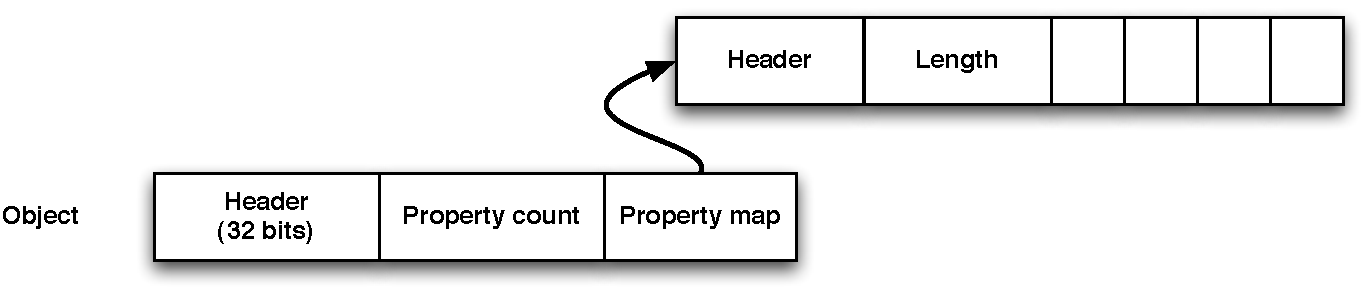
\includegraphics[width=3.5in]{images/obj_layout_basic}
\end{center}
\end{frame}
% ------------------------------------------------------------------------------

% -- Slide ---------------------------------------------------------------------
\begin{frame}
\frametitle{\bf Array Object Layout}

\begin{center}
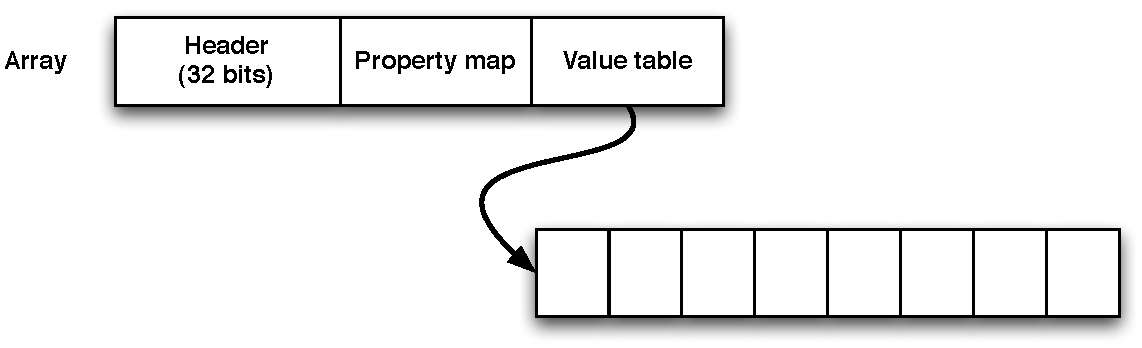
\includegraphics[width=4in]{images/obj_layout_array}
\end{center}
\end{frame}
% ------------------------------------------------------------------------------

% -- Slide ---------------------------------------------------------------------
\begin{frame}
\frametitle{\bf Function Object Layout}

\begin{center}
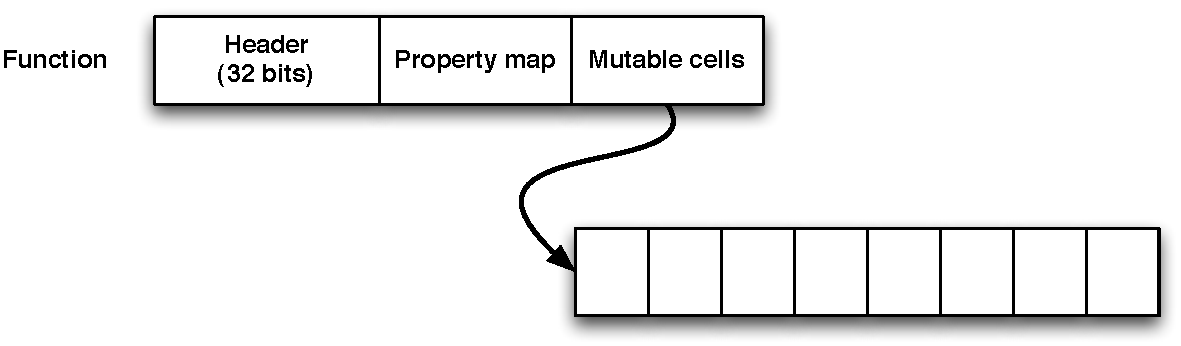
\includegraphics[width=4in]{images/obj_layout_func}
\end{center}
\end{frame}
% ------------------------------------------------------------------------------

% -- Slide ---------------------------------------------------------------------
\begin{frame}
\frametitle{\bf String Object Layout}

\begin{center}
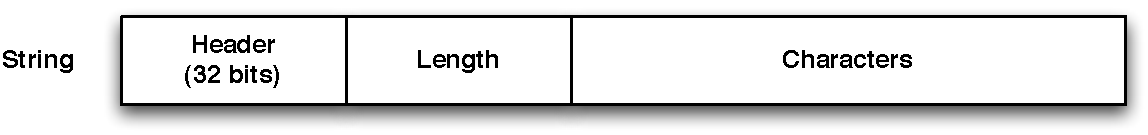
\includegraphics[width=4in]{images/obj_layout_str}
\end{center}
\end{frame}
% ------------------------------------------------------------------------------

% % -- Slide ---------------------------------------------------------------------
% \begin{frame}
% \frametitle{\bf Memory management}
% 
% % - Allocator
% % - Executable code
% \end{frame}
% % ------------------------------------------------------------------------------

% % -- Slide ---------------------------------------------------------------------
% \begin{frame}
% \frametitle{\bf Meta-circularity}
% 
% % - Standard library
% % - Primitives
% % - FFI as bridge
% % - Memory access
% %   - Pointers representation
% %   - Memory block
% % - Numbers
% %   - Representation limits
% \end{frame}
% % ------------------------------------------------------------------------------

% -- Slide ---------------------------------------------------------------------
\begin{frame}
\frametitle{\bf Limitations of JS for compiling writing}

    \begin{itemize}
        \item Limited precision in number representation
        \begin{itemize}
            \item e.g. 64-bit precision numbers
        \end{itemize}
        \item Minimal standard library
        \begin{itemize}
            \item No standard data structures
        \end{itemize}
        \item Bitwise operations limited to 32 bits
        \item Unpredictable allocation behaviour of common operations
        \item Lack of modules
        \item No standard I/O operations
        \item No direct access to memory
    \end{itemize}
\end{frame}
% ------------------------------------------------------------------------------

% % -- Slide ---------------------------------------------------------------------
% \begin{frame}
% \frametitle{\bf Experience}
% 
% % - Dynamicity and testing/refactoring
% % - Metacircularity and intuitive understanding of the language usage patterns
% \end{frame}
% % ------------------------------------------------------------------------------

% -- Slide ---------------------------------------------------------------------
\begin{frame}
\frametitle{\bf Performance - Sunspider Cflow Recursive}

\begin{center}
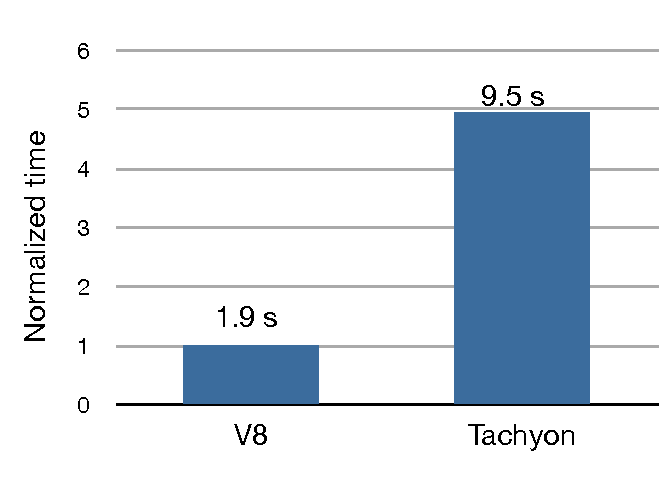
\includegraphics[width=3in]{images/perf-sunspider}
\end{center}

                          % Sunspider control flow recursive (200 iterations)
% - Compilation Time  :   0.8 s tachyon, 0.82 s v8 (combined) 
% - Execution Time    :   5.0 s tachyon,
% - Bootstrapping Time: 6 mins v8, ~1hr tachyon
%                       40-50 gb heap (no gc)
%                       v8 < 1 gb

% d8 version 3.2.3.1
\end{frame}
% ------------------------------------------------------------------------------

% -- Slide ---------------------------------------------------------------------
\begin{frame}
\frametitle{\bf Ballpark Performance Comparison on \code{fib(38)}}

\begin{center}
\rowcolors{1}{RoyalBlue!10}{RoyalBlue!5}
\begin{tabular}{lll}
Tachyon     & 8.110s & (7.20x) \\
WebKit INT  & 7.334s & (6.51x) \\
WebKit      & 1.406s & (1.25x) \\
V8          & 1.127s & (1.00x) \\
gcc -O2     & 0.626s & (0.56x) \\
gcc -O3     & 0.224s & (0.20x)
\end{tabular}
\end{center}

\end{frame}
% ------------------------------------------------------------------------------

% -- Slide ---------------------------------------------------------------------
\begin{frame}
\frametitle{\bf Performance - Tachyon Bootstrap}

\begin{center}
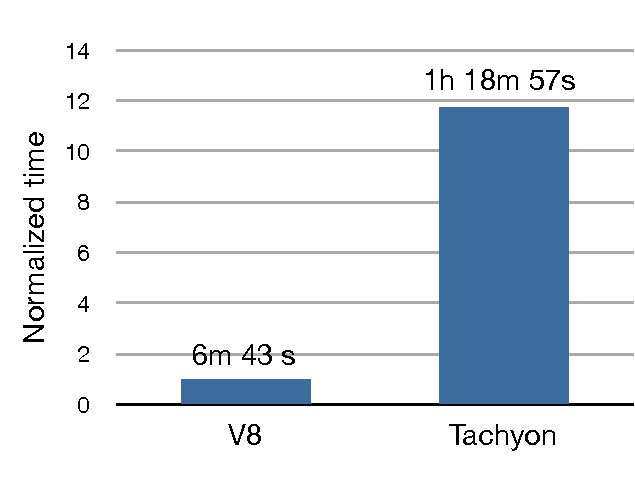
\includegraphics[width=3in]{images/perf-bootstrap}
\end{center}
\end{frame}
% ------------------------------------------------------------------------------

% -- Slide ---------------------------------------------------------------------
\begin{frame}
\frametitle{\bf Allocated Memory - Tachyon Bootstrap}

\begin{center}
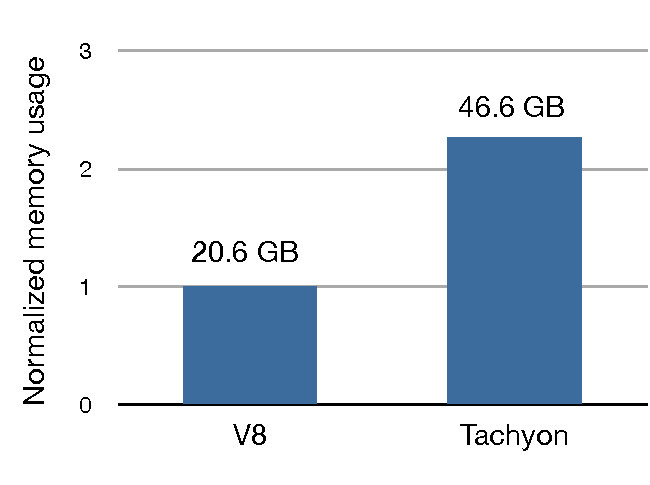
\includegraphics[width=3in]{images/perf-bootstrap-mem}
\end{center}
\end{frame}
% ------------------------------------------------------------------------------
